\subsection{XGBoost}\label{sec:xgb}
One note-worthy classification method is \emph{Gradient Boosting} and its implementation by Tianqi Chen and Tong Hel via the package \emph{XGBoost}.
After sharing it with other participants early in the challenge, they were rewarded with a special jury-award, for providing "a good compromise between performance and simplicity"\cite{HEPml}. While describing XGBoost, we evaluate this method by these criteria.
For own testing, we use the python package of XGBoost version 0.47 available at \url{https://github.com/dmlc/xgboost}, released on 15. Jan. 2016.

\subsubsection{Classification method}
Assuming, we fit a model to solve a problem. Because our solution is not perfect, we expect an error in our prediction. Therefore, we train another model to fit the error.
Gradient Boosting uses this simple concept: We fit one or more models to \emph{fix} our prediction on the training set.
In general, we can express gradient boosting as the optimization problem

\begin{equation}\label{eq:gradboost}
	L(\varnothing)= \sum\limits_{i=1} l ( y_i,(\hat{y}_i + f(x_i)))
\end{equation}, where \emph{l} is a loss-function, $y_i$ and $\hat{y}_i$ the \emph{true} and \emph{predicted} label and $f$ a second, \emph{fixing} model.

The more complex a classification-model is, the the higher is the chance of overfitting. Considering this, the main difference of XGBoost to other gradient boosting classifiers is the simple idea to penalize complex models in the ensemble. By adding a regularization-term $\Omega(f)$ to the objective function (Eq.\eqref{eq:gradboost}), training this model minimizes not only the loss function, but also $\Omega(f_t)$.
The actual predictions are made by weighted \emph{decision trees} with a chosen maximum depth. The tree displayed in Fig. \ref{fig:tree} is one of 100 trees fitted to the original training data with a maximum depth of 3.

\begin{figure}[h]
\begin{center}
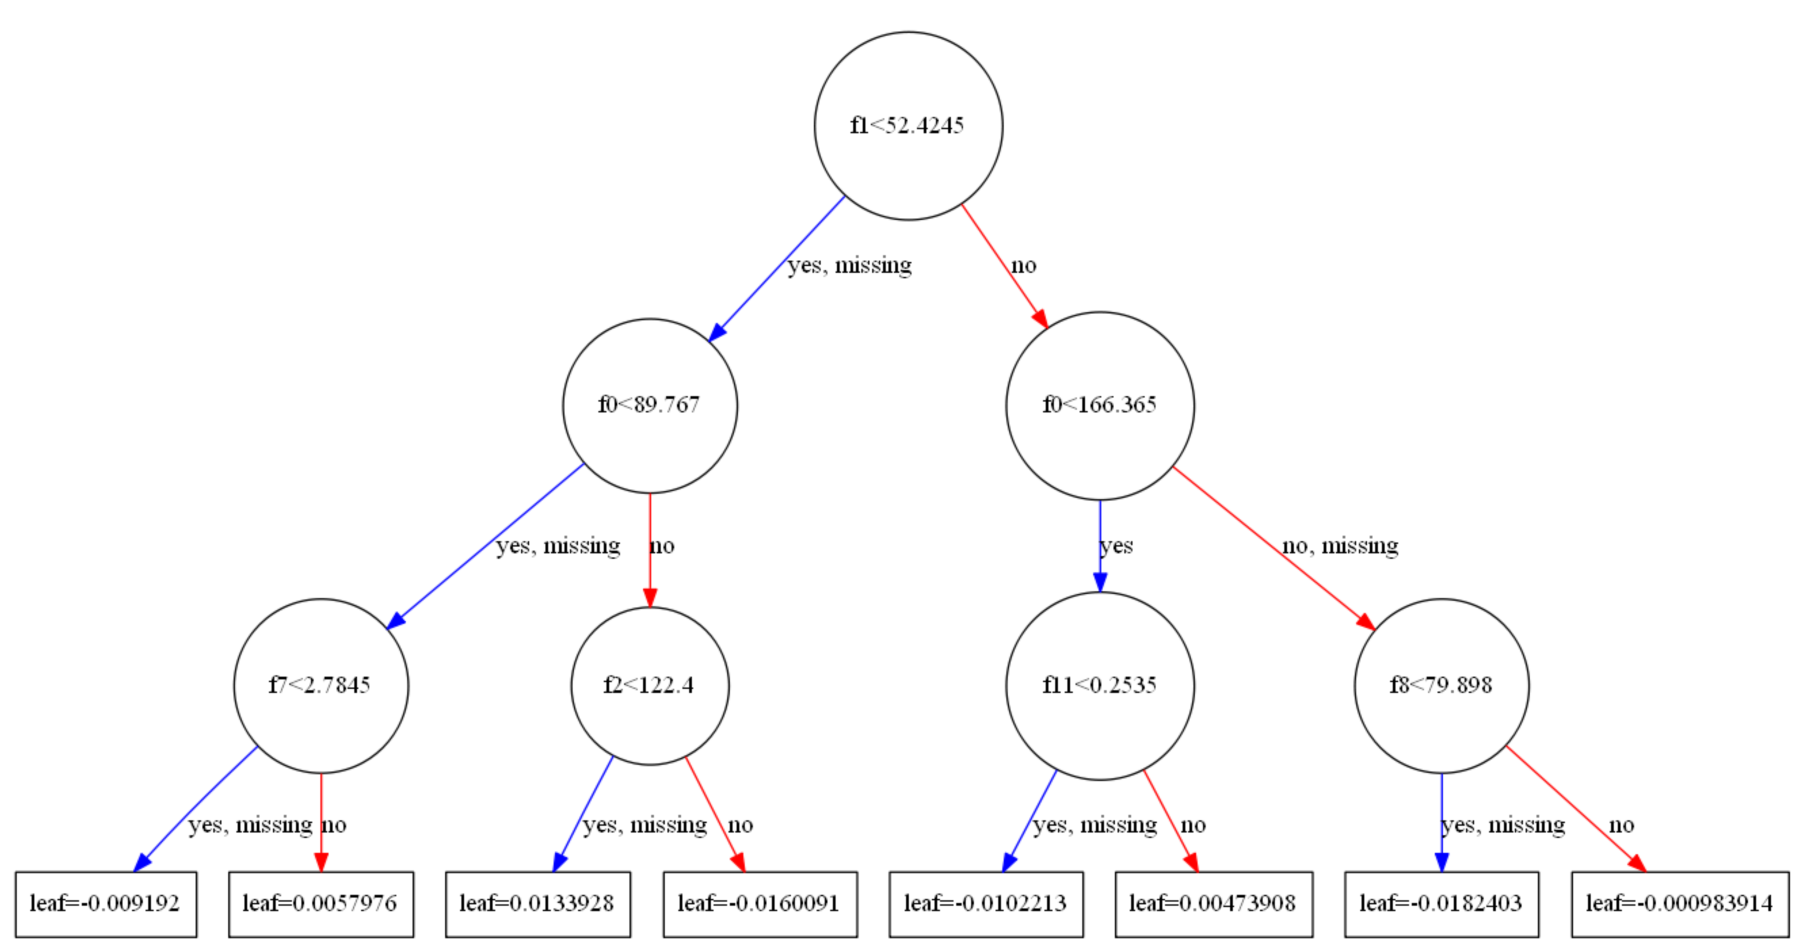
\includegraphics[width=\textwidth]{images/tree}
\caption{A decision tree, visualized by the \emph{plot\_tree}-method included in XGBoost}
\label{fig:tree}
\end{center}
%\vspace{1ex}
\end{figure}

\subsubsection{Performance and optimization}
Using default settings, 100 trees and AMS evaluation, XGBoost achieves a public AMS of about 3.32 using the complete, original data set. We are able to get a significantly higher AMS by tuning parameters, mainly increasing the number of trees up to 3000 and lowering \emph{eta}. Latter parameter determines the \emph{step size shrinkage} to prevent overfitting. Testing shows that eta is inversely related to treenumber, the more trees are used for training, the lower should eta be chosen.
Using all parameters, we are still not able to reproduce the exact AMS on the original data, stated in \cite{chen14}.
Cutting phi-values, which is suggested by some competitors that use XGBoost \cite{blog}, does not improve the results. Further feature selection fails to resolve into better AMS. Adding artificial features works beneficial for several submissions using the method.\\
In its recent version, XGBoost provides several alternative objection function and evaluation-metrics. As the package has been developed for the Kaggle challenge, it also contains AMS and AUC as metrics. While the original submission used AUC as model evalutation, we use AUC \emph{and} AMS for training XGBoost with no noticeable disadvantages.

Many software packages implement gradient boosting, as it is an established method in machine learning. While Fig. \ref{fig:xgb-speed} compares speed-benchmarks, with all algorithms set up to fit 120 trees with depth 6 and \emph{eta}=0.1, we consider AMS as it is the main-goal of the challenge. Since our own approaches rely on scikit-learn, we compare the performance of the \emph{GradientBoostingClassifier}(GBC)-class to XGBoost , see Fig. \ref{fig:xgb-gbc}.\\
The training time of GBC consumes over 5000 seconds, while using 100 trees of depth 12. We pass on performing further training of GBC with more trees. However, it is worth mentioning that the longest training, that was performed on a XGBoost classifier for this Thesis, terminated after 1666 seconds, calculating 3000 trees with a depth of 12.
By preprocessing the mathematical model and using decision trees, the training complexity for a tree is reduced to $O(ndK)$ for \emph{n} samples with \emph{d} features, where \emph{K} is the maximum depth of a decision tree.

\begin{figure}[h]
\centering
\begin{minipage}{0.48\textwidth}
  \centering
  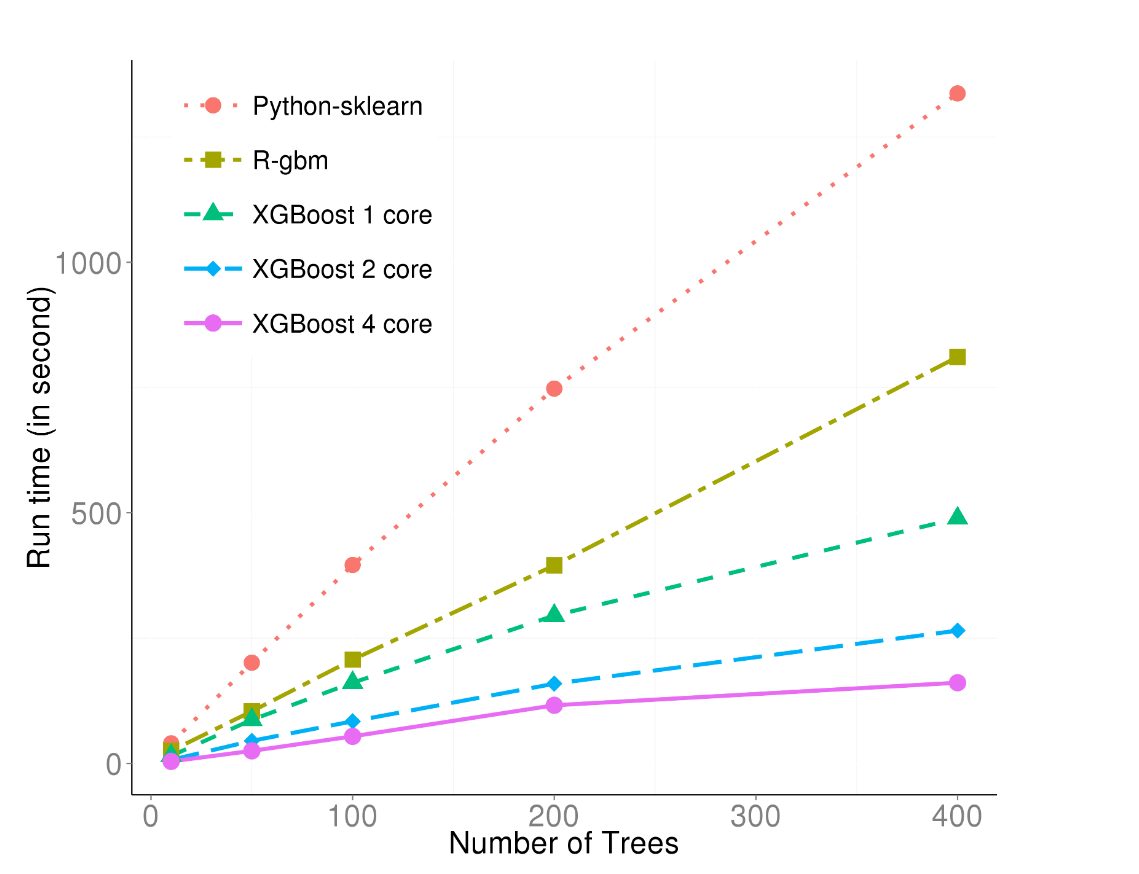
\includegraphics[width=\linewidth]{images/xgboost-speed}
  \vspace{-0.1ex}
	\caption{\\Speed Benchmark on challenge data \cite{chen14}}
	\label{fig:xgb-speed}
\end{minipage}
\quad
\begin{minipage}{0.48\textwidth}
  \centering
  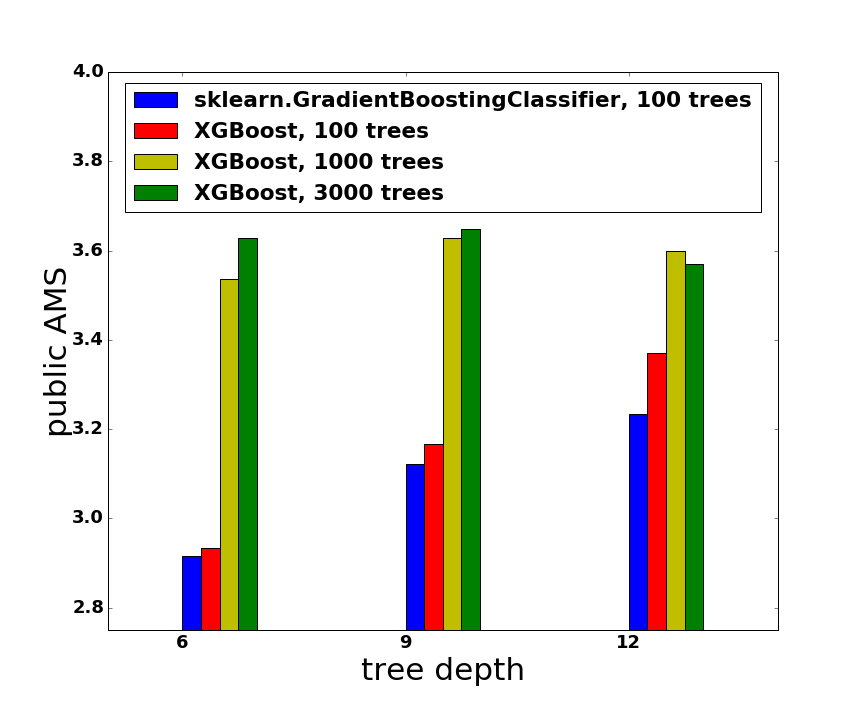
\includegraphics[width=\linewidth]{images/xgb-gbc}
	\caption{\\AMS-Comparison XGBoost and sklearn.GradientBoostingClassifier}
	\label{fig:xgb-gbc}
\end{minipage}
%\vspace{1ex}
\end{figure}

Regarding the special award, XGBoost seems to fulfil every of its defined aspects. While many other submissions outperform the best benchmark \emph{MultiBoost} easily aswell, this package does it remarkably fast. Training time for a benchmark-surpassing result takes under 37 seconds with tuned parameters, using up to 8 CPU threads. This specific run achieved a public AMS of 3.5399.
The developers made the package available early in the challenge, many other participants used it at some point to test custom feature sets or benchmark their own approaches.

It is justified to acknowledge this package, as it could have impact on tools, which are being used in high-energy physics\cite{HEPml}.
